\documentclass[UTF8]{ctexart}
%\documentclass[a4paper]{article}
% \usepackage[margin=1.25in]{geometry}
\usepackage[inner=2.0cm,outer=2.0cm,top=2.5cm,bottom=2.5cm]{geometry}
%\usepackage{CJK}
\usepackage{color}
\usepackage{graphicx}
\usepackage{amssymb}
\usepackage{amsmath}
\usepackage{amsthm}
\usepackage{bm}
\usepackage{hyperref}
\usepackage{multirow}
\usepackage{enumerate}
\usepackage{listings}
\usepackage{xcolor}
\usepackage{fontspec}
\setmainfont{Times New Roman}

\newcommand{\homework}[5]{
    \pagestyle{myheadings}
    \thispagestyle{plain}
    \newpage
    \setcounter{page}{1}
    \noindent
    \begin{center}
    \framebox{
        \vbox{\vspace{2mm}
        \hbox to 6.28in { {\bf 操作系统 \hfill #2} }
        \vspace{6mm}
        \hbox to 6.28in { {\Large \hfill #1 \hfill} }
        \vspace{6mm}
        \hbox to 6.28in { {\it 指导老师: {\rm #3} \hfill 姓名: {\rm #4},学号: {\rm #5}}}
        \vspace{2mm}}
    }
    \end{center}
    % \markboth{#4 -- #1}{#4 -- #1}
    \vspace*{4mm}
}


\newcommand{\yahei}{\setCJKfamilyfont{yahei}{Microsoft YaHei} \CJKfamily{yahei}}




\newenvironment{solution}
{\color{blue} \paragraph{Solution.}}
{\newline \qed}

\begin{document}


%大标题在这里改!!!!!!!!!
\homework{L0实验报告}{2020 春}{蒋炎岩}{杨旖纯}{181220064}

\lstset{numbers=left,numberstyle=\tiny,keywordstyle=\color{blue!70},commentstyle=\color{red!50!green!50!blue!50},frame=shadowbox, rulesepcolor=\color{red!20!green!20!blue!20},escapeinside=``,xleftmargin=2em,xrightmargin=2em, aboveskip=1em}



\paragraph{前言}
    你可以把写在前面的话写在这里
~\\
\section{说明}
    我担心你很多命令不清楚,所以把自己会的东西都展示了一遍,你依葫芦画瓢就行。

    有问题随时QQ戳我哦

默认是宋体

\it 这是楷体

\bf 这是加粗

{\fangsong 这是仿宋}

{\heiti 这是黑体}

{\yahei 这是微软雅黑}

\rm % 将环境恢复为宋体
~\\
\section{这是一级标题}
\subsection{这是二级标题}
\subsubsection{这是三级标题}

\section{插入图片的方法}%图片需要和.tex文件同一目录才行。
\begin{figure}[ht]
    \centering
    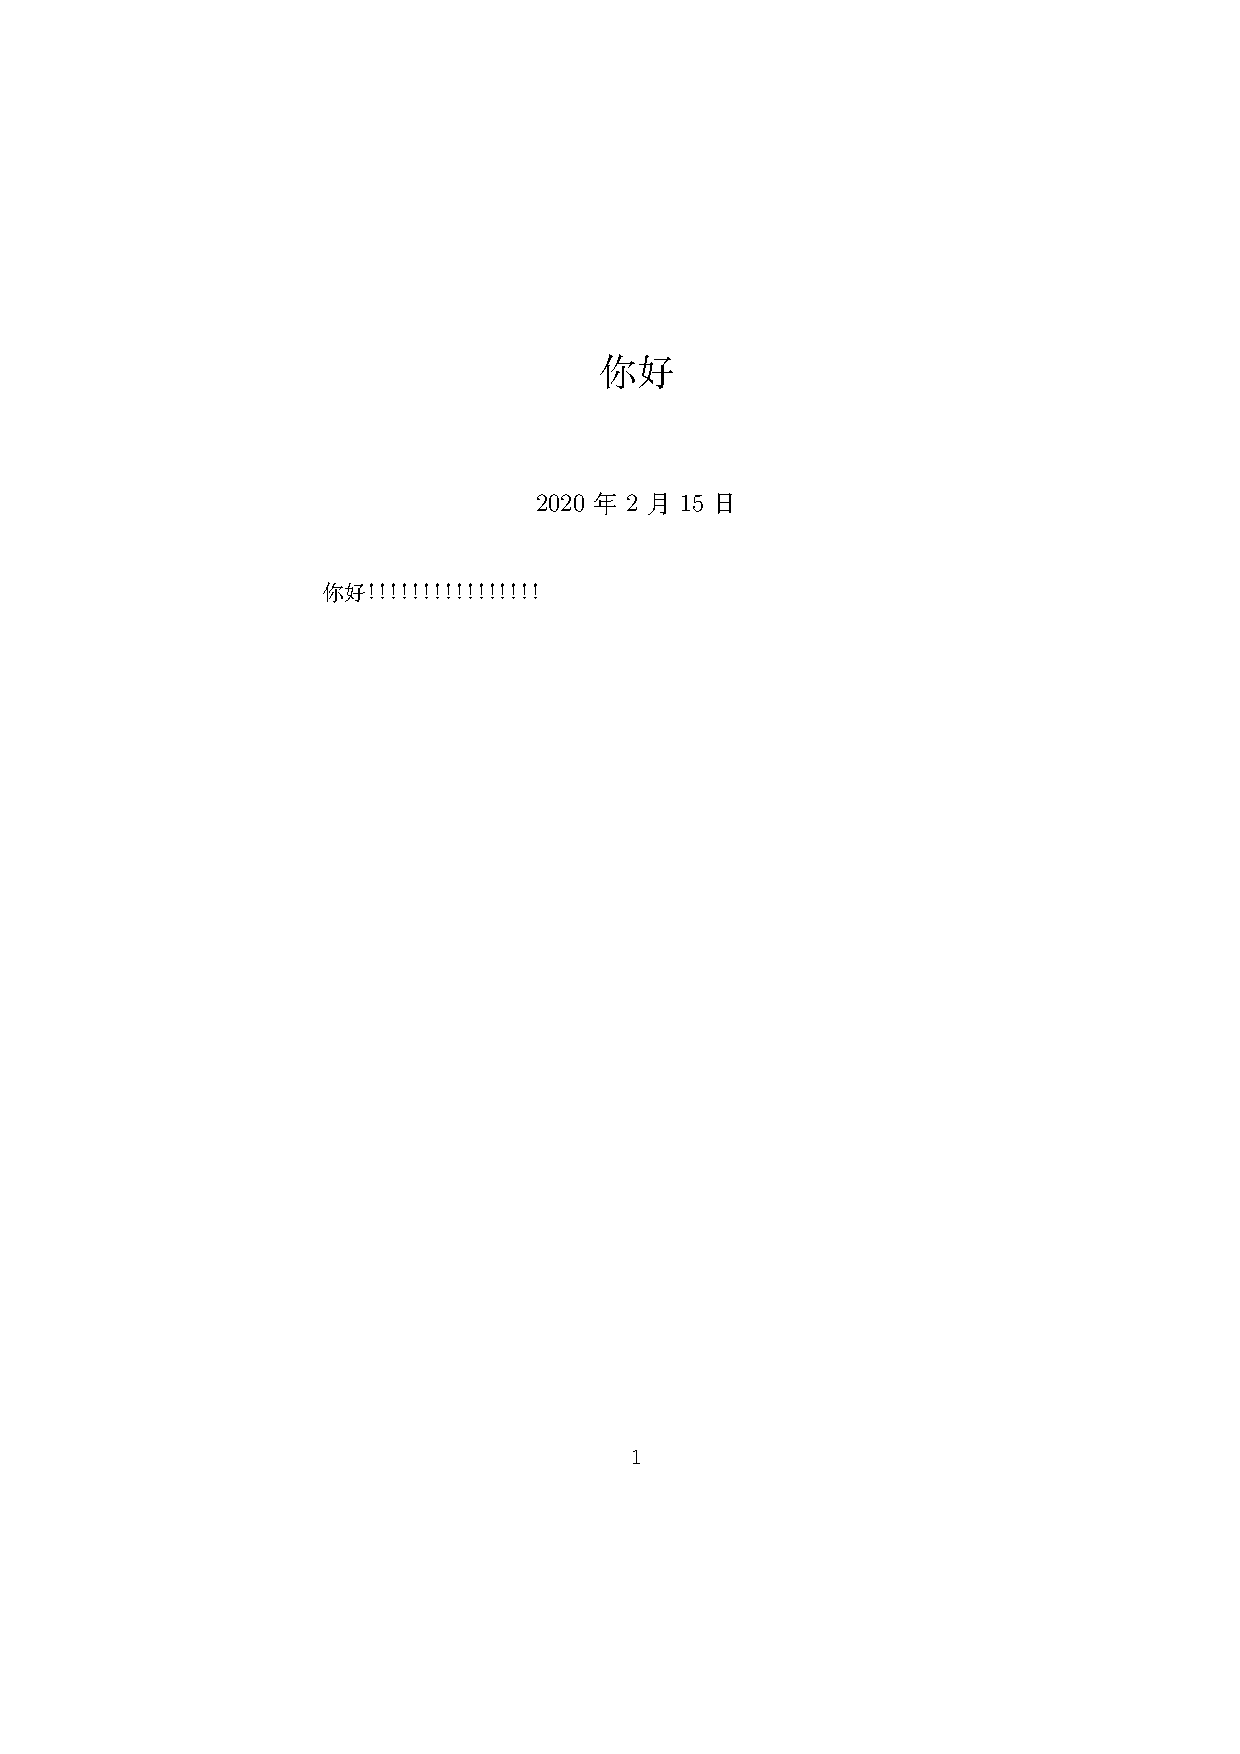
\includegraphics[scale=0.2]{test.jpg}%还有height width等可选参数
    \caption{这是一张图片哦,给她取个名字~}
    \label{fig:test}%做一个标签
\end{figure}


~\\
~\\

\section{把你想插入的代码放在这个下面}
\begin{lstlisting}[language={[ANSI]C}]
   #include <stdio.h>
   int main()
   {
       printf("Hello!");
   }

\end{lstlisting}
\section{一个例子}
    相比过程抽象,数据抽象将front,rear等指示循环数组头尾的重要信息封装了起来,数据与功能联系紧密,防止无关的外部函数对其进行操作,避免了可能存在的函数副作用对数据的影响。而过程抽象的实现将front与rear定义为全局变量,数据与功能联系松散,一方面让模块的划分更加模糊,另一方面也造成了潜在的在未来编写其他函数或变量时,因强符号、弱符号的区别造成意想不到的符号重定义、语义与实际链接对象不符等链接错误。
    爱仕达所多
    相比过程抽象,数据抽象将front,rear等指示循环数组头尾的重要信息封装了起来,数据与功能联系紧密,防止无关的外部函数对其进行操作,避免了可能存在的函数副作用对数据的影响。而过程抽象的实现将front与rear定义为全局变量,数据与功能联系松散,一方面让模块的划分更加模糊,另一方面也造成了潜在的在未来编写其他函数或变量时,因强符号、弱符号的区别造成意想不到的符号重定义、语义与实际链接对象不符等链接错误。
    爱仕达所多

    相比过程抽象,数据抽象将front,rear等指示循环数组头尾的重要信息封装了起来,数据与功能联系紧密,防止无关的外部函数对其进行操作,避免了可能存在的函数副作用对数据的影响。而过程抽象的实现将front与rear定义为全局变量,数据与功能联系松散,一方面让模块的划分更加模糊,另一方面也造成了潜在的在未来编写其他函数或变量时,因强符号、弱符号的区别造成意想不到的符号重定义、语义与实际链接对象不符等链接错误。
    爱仕达所多

    相比过程抽象,数据抽象将front,rear等指示循环数组头尾的重要信息封装了起来,数据与功能联系紧密,防止无关的外部函数对其进行操作,避免了可能存在的函数副作用对数据的影响。而过程抽象的实现将front与rear定义为全局变量,数据与功能联系松散,一方面让模块的划分更加模糊,另一方面也造成了潜在的在未来编写其他函数或变量时,因强符号、弱符号的区别造成意想不到的符号重定义、语义与实际链接对象不符等链接错误。
    爱仕达所多

    相比过程抽象,数据抽象将front,rear等指示循环数组头尾的重要信息封装了起来,数据与功能联系紧密,防止无关的外部函数对其进行操作,避免了可能存在的函数副作用对数据的影响。而过程抽象的实现将front与rear定义为全局变量,数据与功能联系松散,一方面让模块的划分更加模糊,另一方面也造成了潜在的在未来编写其他函数或变量时,因强符号、弱符号的区别造成意想不到的符号重定义、语义与实际链接对象不符等链接错误。
    爱仕达所多

    相比过程抽象,数据抽象将front,rear等指示循环数组头尾的重要信息封装了起来,数据与功能联系紧密,防止无关的外部函数对其进行操作,避免了可能存在的函数副作用对数据的影响。而过程抽象的实现将front与rear定义为全局变量,数据与功能联系松散,一方面让模块的划分更加模糊,另一方面也造成了潜在的在未来编写其他函数或变量时,因强符号、弱符号的区别造成意想不到的符号重定义、语义与实际链接对象不符等链接错误。
    爱仕达所多

    相比过程抽象,数据抽象将front,rear等指示循环数组头尾的重要信息封装了起来,数据与功能联系紧密,防止无关的外部函数对其进行操作,避免了可能存在的函数副作用对数据的影响。而过程抽象的实现将front与rear定义为全局变量,数据与功能联系松散,一方面让模块的划分更加模糊,另一方面也造成了潜在的在未来编写其他函数或变量时,因强符号、弱符号的区别造成意想不到的符号重定义、语义与实际链接对象不符等链接错误。
    爱仕达所多


\end{document}
